\section{Method \& Theory}\label{sec:method_theory}
In this chapter we give an overview of the theory and methods which are used throughout the investigations. We begin in section \ref{sec:cmd_theory} with the description of the stellar population of a \ac{GC}. In \ref{sec:kin_prof_theory} we then explain the kinematic properties, i.e. velocity dispersion and anisotropy parameter. Still in phase space in section \ref{sec:dens_pot_theory} we introduce density and different potential models. In the next section \ref{sec:iof} we define orbits and their classical integrals of motion. After explaining the benefit of the effective potential in section \ref{sec:pot_eff} we show how we calculate the actions as best choice of integrals of motions(section \ref{sec:actions}). Then we give the numerical way of calculating orbits (section \ref{sec:num_int}) for which we give some examples in the last part \ref{sec:orbit_examples} of this chapter. If not said else we define all properties as specific ones which means they are given in units of the mass of the star.
\subsection{Stellar population in GC}\label{sec:cmd_theory}
The typical stellar population of a \ac{GC} can be seen in a \ac{CMD}. We show in figure \ref{fig:cmd} an example of a \ac{CMD} extracted from one of our simulations (SIM 1, described in section \ref{sec:description}). In this \ac{CMD} the absolute V-band magnitude is plotted against the B-V color. The color code indicates the mass of the stars. 
\begin{figure}[htbp]
\centering
	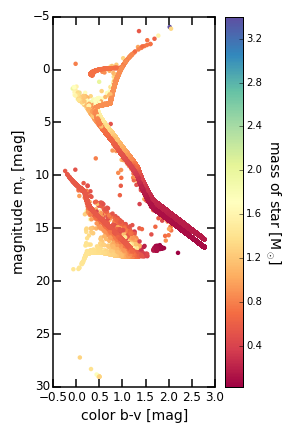
\includegraphics[width=0.5\textwidth]{Plots/color_magnitude_diagram.png}
	\caption{Color magnitude diagram of SIM 1. The absolute V-band magnitude versus the color B-V gives us an overview of the stellar population of this \ac{GC}. The stars are color coded by their masses. On the main sequence there are two branches. These are caused by binary systems. Following the main sequence there is the turn-off. Going further blue struggles are located. Right to the turn-off there is the sub giant branch followed by the red giant branch. The most luminous stars are situated on the early asymptotic giant branch. At a absolute magnitude of zero there is the horizontal branch where stars burn He quiescently. Below  the main sequence and blue stragglers the white dwarfs are located. Having nearly no luminosity dark stellar remnants are situated at the bottom of the \ac{CMD}.}
	\label{fig:cmd}
\end{figure}
The position of a star in the \ac{CMD} can be interpreted as its evolution stage. Most of the stars are in the main sequence and they are characterized by hydrogen fusion in their cores. There are two main sequence lines one upon the other. These occur due to binary systems whose flux is given by the sum of the single fluxes of the single components, and therefore appear redder and more luminous. These binary systems represent about \unit[7.5]{\%} of the stars in the \ac{GC}. The position of the main sequence turn-off depends on the age of the system and therefore can be used as an indicator to determine the age of the cluster. Isochrones are curves of evolutionary stages of stars of a \ac{SSP} having the same age and metallicity but different masses. Bluewards of this turn off point, following the trend of main sequence stars, there are so called "blue stragglers" which are remnants of stellar collisions or interacting binaries \citep[p.628]{2008gady.book.....B}. Continuing from the turn off point there are the sub giant and the red giant branch consisting of stars still fusing hydrogen but only in a shell surrounding a degenerate helium core. They are inflated with a radius much higher than the main sequence stars but have a much lower surface temperature. On the early asymptotic giant branch following the red giant branch the stars are burning helium in their shells. These are the brightest stars of a \ac{GC}. On the upper part of the red giant branch lies the horizontal branch. Its stars burn helium in their core and hydrogen in a surrounding shell. In the lower left corner white dwarfs are located. They are stellar remnants which have burnt all of their resources. In a typical \ac{GC} dark stellar remnants like stellar black holes and neutron stars are present but not visualised in the \ac{CMD}. In this \ac{CMD} we see them at the bottom of the figure. \cite[p.476-477]{2006ima..book.....C}.
\subsection{Kinematic profiles of globular clusters}\label{sec:kin_prof_theory}
We will investigate \acp{GC} in phase space by analysing the stellar kinematic profiles (such as velocity dispersion and anisotropy profiles) and the spatial distribution of stars (density profiles and potential). 
\par The stellar velocity dispersion quantifies the spread of different velocities stars at given positions can have. With the actual velocity \(\mathrm{v_i}\) of the i-th star, \(\left\langle \mathrm{v}\right\rangle\) specifying the mean of the velocities of all considered N stars and the mean of the n-th power of the total velocity given by
\begin{equation}
\mathrm{\left\langle \mathrm{v^n}\right\rangle=\frac{1}{N}\sum_{i=1}^Nv_i^n}
\end{equation}
 we can calculate the velocity dispersion as the standard deviation of the velocity distribution: 
\begin{equation}\label{eq:vel_disp}
\sigma_\mathrm{i}(\mathrm{r})\equiv\sqrt{\left\langle(\mathrm{v_i}(\mathrm{r})-\langle \mathrm{v_i}(\mathrm{r})\rangle)^2\right\rangle}=\sqrt{\left\langle \mathrm{v_i}(\mathrm{r})^2\right\rangle-\langle \mathrm{v_i}(\mathrm{r})\rangle^2} \qquad\qquad \mathrm{i=r,\theta,\phi}.
\end{equation}  For a spherical system it is best to calculate them in spherical coordinates \(\mathrm{r},\theta,\phi\) respectively \(\mathrm{v_r,v_{\theta},v_{\phi}}\). If the \ac{GC} contains an \ac{IMBH} the velocity dispersion towards the centre is expected to increase. 
\par The direction of the motion of a star can be described by its anisotropy. In a spherical system we compare the motion in radial direction to the motion in sperical shells at the given distance of the star. The dispersions of motions are described by equation \ref{eq:vel_disp}. To quantify the anisotropy of the system we use the anisotropy parameter \(\beta\) 
\begin{equation}\label{eq:anisotropy}
\mathrm{\beta(r)\equiv1-\frac{\sigma_\theta ^2(r)+\sigma_\phi ^2(r)}{2\sigma_r ^2(r)}}
\end{equation} taken from \citet[eq. 4.61]{2008gady.book.....B}. There the numerator describes the dispersion of motions on the spherical shell while the denominator is given by the squared radial dispersion. If \(\beta\) is positive the anisotropy is radial i.e. the velocity dispersion is larger in radial direction than in tangential direction, if it is negative the anisotropy is tangential and if \(\beta\approx0\) then the system is isotropic that means the stars have random motions in all directions at the same rate. 
\subsection{Density \& potential}\label{sec:dens_pot_theory}
\subsubsection{Density of a collisionless stellar system}\label{sec:density}
We calculate the mass density of the \acp{GC} by binning the masses on logarithmic equally distributed shells
\begin{equation}\label{eq:density}
\rho(\mathrm{r})=\frac{\sum_{\mathrm{r=r_{in}}}^{\mathrm{r_{out}}}\mathrm{M(r)}}{\mathrm{V(r_{out}-r_{in})}}=\frac{3}{4\pi}\frac{\sum_{\mathrm{r=r_{in}}}^{\mathrm{r_{out}}}\mathrm{M(r)}}{\mathrm{r_{out}^3-r_{in}^3}}
\end{equation} 
with the sum of masses of stars with mass M(r) over a volume V which is taken from the radius of the inner shell \(\mathrm{r_{in}}\) and the radius of the outer shell \(\mathrm{r_{out}}\). 
\par We consider \acp{GC} as quasi-collisional stellar system but can approximate them as collisionless motivated by the fact that the dynamical time of a cluster is always shorter than the relaxation time \(\mathrm{T_{dyn} < T_{relax} < T_{ageGC} \equiv T_{Hubble}}\). \(\mathrm{T_{dyn}}\) is the time of a star to go from one side of the cluster to the other. This takes approximately \unit[10\(^5\)]{yr}. The relaxation time is the time needed to redistribute energies of the stellar encounters and takes about \unit[10\(^7\) - 10\(^9\)]{yr}. The age of the \acp{GC} is approximately the Hubble time which is the age of the universe (\unit[10\(^{10}\)]{yr}). The first term motivates the collisionless approximation while the part starting with \(\mathrm{T_{relax}}\) is telling us that a \ac{GC} has lived for several relaxation times, therefore two-body interaction had time to act. That means in the long term that the system is collisional. 
\subsubsection{Generating the potential from Poisson's equation}\label{sec:poisson}
If the system is spherical symmetric the potential and force depend only on the distance from the centre r. Under the condition that the system is collisionless the potential \(\Phi\) can be derived from the Poisson's equation \begin{equation}\label{eq:Poisson}
\mathrm{\Delta\Phi(r)=4\pi G \rho(r)}
\end{equation}
with the gravitational constant G = \unitfrac[\(6.674\cdot10^{-11}\)]{\(\mathrm{m}^3\)}{\(\mathrm{kg\ s}^2\)} \citep{2015arXiv150707956M} and the density \(\rho\) depending only on the distance as well. In general one can use the Poisson's equation for every system but then it is depending on the position vector \(\vec{\mathrm{x}}\). 
\par Due to the spherical symmetry the potential can be calculated by 
\begin{equation}\label{eq:numerical_poisson}
\mathrm{\Phi(r)=-\frac{G}{r}\int_0^r{\mathrm{d}M(r')}-G\int_r^{\infty}{\frac{\mathrm{d}M(r')}{r'}}=-4\pi G\left[\frac{1}{r}\int_0^r\mathrm{d}r'r'^2\rho(r')+\int_r^{\infty}\mathrm{d}r'r'\rho(r')\right]}
\end{equation} with dM describing the mass of spherical shells as proved by \citet[eq. 2.28]{2008gady.book.....B}. 
\subsubsection{Other potential models}\label{sec:other_pot}
One of the most simple potentials is the Kepler potential. It describes the potential given by a point mass M
\begin{equation}\label{eq:kep_pot}
\mathrm{\Phi(r)=-\frac{GM}{r}}
\end{equation}  taken from \citet[eq. 2.34]{2008gady.book.....B}. The potential generated by the \acp{IMBH} can be described  as Keplerian. 
\par Another description of spherical systems is given by the Plummer model. It is based on the assumption that the density is nearly constant in the centre and equals zero at large radii. The given potential is 
\begin{equation}\label{eq:Plum_pot}
\mathrm{\Phi(r)=-\frac{GM}{\sqrt{r^2+b^2}}}
\end{equation}
\citep[eq. 2.44a]{2008gady.book.....B} where M is the total mass of the system and b is the Plummer scale length. In \citet{1911MNRAS..71..460P} Plummer used this potential to describe observations of \acp{GC}. the corresponding density to this model is given by \citet[eq. 2.44b]{2008gady.book.....B}
\begin{equation}\label{eq:Plumm_dens}
\mathrm{\rho(r)=\frac{3M}{4\pi b^3}\left(1+\frac{r^2}{b^2}\right)^{-\frac{5}{2}}.}
\end{equation}
This model cannot be used to describe the position of a star on its orbit in elementary functions. 
\par In \citet{2014arXiv1411.4937B} he claims that \acp{GC} can be described by an isochrone (see section \ref{sec:cmd_theory}) potential 
\begin{equation}\label{eq:isochr_pot}
\mathrm{\Phi(r)=-\frac{GM}{b+\sqrt{b^2+r^2}}}
\end{equation} 
\citep[eq. 2.47]{2008gady.book.....B}. This model delivers analytical functions for the properties of orbits.
\subsection{Orbits \& integrals of motion}\label{sec:orbit_int_of_motion_theory}
\subsubsection{Classical integrals of motion in spherical potential}\label{sec:iof}
If a tracer particle, e.g. a star, moves freely in a gravitational potential generated by a mass distribution its path in 6D position-velocity space (\(\vec{\mathrm{x}}(\mathrm{t}),\vec{\mathrm{v}}(\mathrm{t})\)) is called "orbit".
How positions and velocities along the orbit are linked contains information about the potential. With Newton's 2nd law we get the connection between potential \(\Phi(\vec{\mathrm{x}})\)and acceleration \(\vec{\mathrm{a}}\) which the star of mass m experiences which is 
\begin{equation}\label{eq:Newton}
\vec{\mathrm{F}}(\vec{\mathrm{x}})=-\nabla\Phi(\vec{\mathrm{x}})=\mathrm{m}\cdot\vec{\mathrm{a}}.  
\end{equation}
Here \(\vec{\mathrm{F}}\) is the force at given position \(\vec{\mathrm{x}}\).
\par Despite the description of orbits in the 6D position velocity space it can be described by integrals of motion which are constant along an unperturbed orbit. A spherical potential allows four conserved quantities, i.e. the classical integrals of motions, which are the energy and the three components of the angular momentum. That restricts the orbits in spherical potentials to happen in a plane. The energy is given by the sum of the kinetic energies in the 3D velocity space and the potential:
\begin{equation}\label{eq:energy}
\mathrm{E(r)=\frac{v_x(r)^2+v_y(r)^2+v_z(r)^2}{2}+\Phi(r)}.
\end{equation}
The total angular momentum
\begin{equation}\label{eq:total_ang_mom}
\vec{\mathrm{L}}=\vec{\mathrm{x}}\times\vec{\mathrm{v}}=\sqrt{L_x^2+L_y^2+L_z^2}
\end{equation}
can be written as superposition of the angular momenta in each direction which are given by 
\begin{equation}\label{eq:ang_mom}
\mathrm{L_k=\varepsilon_{klm}x_l v_m}
\end{equation}
where \(\mathrm{\varepsilon_{klm}}\) is the Levi-Civita symbol.  
\par On a perturbed orbit, e.g. numerical fluctuations near the \ac{IMBH}, integrals of motion can vary and evolve a time dependency. We assume that the stars move along unperturbed orbits. 
\subsubsection{The effective potential}\label{sec:pot_eff}
The effective potential \(\mathrm{\Phi_{L}(r)}\) (see figure \ref{fig:pot_eff_theory}) describes the potential a star with given angular momentum L experiences in a gravitational potential  \(\Phi(\mathrm{r})\):
\begin{equation}\label{eq:eff_pot}
\mathrm{\Phi_L(r)=\Phi(r)+\frac{L^2}{2r^2}}.
\end{equation} 
which is dependent on the Centrifugal potential \(\mathrm{L^2/2r^2}\) (taken from \citet[p. 59, eq. 6.27]{bartelmann}). 
\begin{figure}[htbp]
\centering
\subcaptionbox{General potential of a central field. The black line is the potential which is the difference between the effective potential (yellow line) and the centrifugal potential (red line). If the effective potential is positive the object is unbound while having a negative potential the object moves on a bound orbit. The points where the effective potential equals the total energy are the peri- and apocentre (r\(_1\) and r\(_2\)) of the orbit. The point with the lowest effective potential is the guiding star radius. This is the distance a star with given angular momentum would have on a circular orbit. \citep[p.59]{bartelmann}\label{fig:eff_potential_bartelmann}}{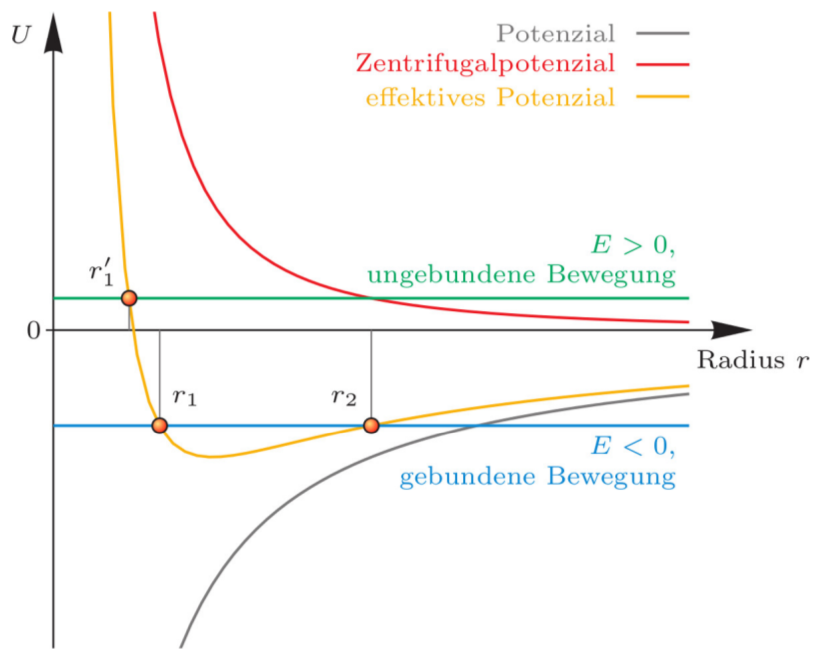
\includegraphics[width=0.475\textwidth]{Plots/eff_potential_bartelmann.png}}
\hfill
\subcaptionbox{Determination of pericentre, apocentre and guiding star radius given by equation \eqref{eq:root_pot_eff}. The intersections of zero and effective potential are the peri- and the apocentre of the star (magenta and black lines) and the minimum of the effective potential (green line) is the guiding star radius .\label{fig:pot_eff_theory_part}}{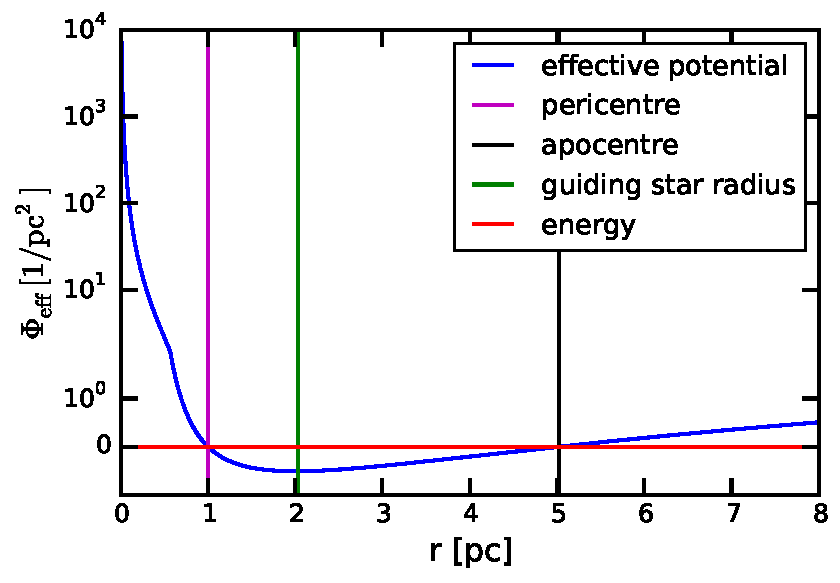
\includegraphics[width=0.475\textwidth]{Plots/pot_eff_theory_part.pdf}}

\caption{Effective potential (panel \subref{fig:eff_potential_bartelmann}) and its form to calculate pericentre, apocentre and guiding star radius (panel \subref{fig:pot_eff_theory_part}).}
\label{fig:pot_eff_theory}
\end{figure}
If the orbit is unbound the effective potential is positive. A star on a bound orbit experiences negative effective potential. 
\par The radii where the bound orbit has the smallest respectively the highest distance to its gravitational centre are called pericentre \(\mathrm{r_{min}}\)  and apocentre \(\mathrm{r_{max}}\).  There the effective potential equals the total energy E since the stars do not have any kinetic energy there. That results in following function (see figure \ref{fig:pot_eff_theory_part}) which is to solve: 
\begin{equation}\label{eq:root_pot_eff}
\mathrm {\Phi(r)-E +\frac{L^2}{2r^2}=0\Rightarrow\left(\frac{1}{r}\right)^2+\frac{2\cdot (\Phi(r)-E)}{L^2}=0.}
\end{equation}
\par The guiding star radius is the distance at which a star with given total angular momentum would have a circular orbit. This is at the minimum of the effective potential. To get \(\mathrm{r_g}\) we have to solve
\begin{equation}\label{eq:min_pot_eff}
\mathrm{\frac{\partial\Phi_L}{\partial r}=\frac{\partial\Phi}{\partial r}-\frac{L^2}{r^3}=0\Rightarrow r\sqrt{r\frac{\partial\Phi}{\partial r}}-|L|=0}
\end{equation} where \(\mathrm{\sqrt{r\frac{\partial\Phi}{\partial r}}=v_{circ}}\) is the circular velocity. This distance is used to have a better comparison of the actions since in the snapshot the stars are at a random position on their orbit.

\subsubsection{Actions}\label{sec:actions}

Stars in spherical symmetric potential are fully described by their actions \begin{equation}
J_i=\frac{1}{2\pi}\oint_{\gamma_i}\vec{p}\cdot d\vec{q} \qquad\qquad i=r,\theta,\phi
\end{equation} which are used as coordinates in action space
These actions are integrals of motion. For most potentials actions can't be described analytically. The actions of a spherical system are derived from angular momentum, energy and potential. Only the potential is depending in r. Energy and angular momentum as well as resulting actions are constant over time and orbit. The azimuthal action J\(_\phi\) and the latitudinal action J\(_\theta\) can be evaluated simply. To calculate the radial action J\(_r\) we have to solve an integral numerically. Actions of a spherical potential are found to be 
\begin{align}\label{eq:actions}
J_\phi=L_z, \\ J_\theta=L-|L_z|, \\ J_r=\frac{1}{\pi} \int_{r_{min}}^{r_{max}} \mathrm{d}r \sqrt{2E-2\Phi(r)-\frac{L^2}{r^2}}. 
\end{align}

\subsubsection{Numerical orbit integration}\label{sec:num_int}
To derive the potential we solve the integrals of the Poisson's equation \eqref{eq:numerical_poisson} numerically by using the Gauss-Legendre quadrature 
\begin{equation}\label{eq:Gauss-Legendre}
\int_a^b f(x)dx \approx \frac{b-a}{2}\sum_{i=1}^n w_i f\left(\frac{b-a}{2}x_i+\frac{a+b}{2}\right)
\end{equation} where the points \(\mathrm{x_i}\) and the weights \(\mathrm{w_i}\) are derived from the Legendre polynomials and a and b are the integration limits. This gives us the numerical formula for the potential 
\begin{equation}\label{eq:numerical_potential}
\begin{aligned}
\Phi(r)= & -4\pi G \cdot \frac{1}{2}\sum_{i=1}^n  w_i\left(\frac{r}{2}x_i+\frac{r}{2}\right)^2\rho\left(\frac{r}{2} x_i+ \frac{r}{2}\right) \\
&-4\pi G\cdot\frac{\infty-r}{2}\sum_{i=1}^n w_i\left(\frac{\infty-r}{2} x_i +\frac{\infty+r}{2}\right)\rho\left(\frac{\infty-r}{2} x_i +\frac{\infty+r}{2}\right)
\end{aligned}
\end{equation}
\par To describe the orbit we need its position and velocity at each time step we use the numerical leapfrog method which is a second-order time reversible integrator. \(X_i\) and \(v_i\) are calculated by 
\begin{align}
x_{i+1}=x_i+v_i\Delta t+\frac{a_i(x_i)}{2}\Delta t^2 \\
v_{i+1}=v_i+\frac{a(x_{i+1})+a(x_i)}{2}\Delta t.
\end{align}
\subsection{Examples for orbits in spherical potentials}\label{sec:orbit_examples}
